\documentclass[tikz,border=8pt]{standalone}
\usepackage[T1]{fontenc}
\usepackage{helvet}
\renewcommand{\familydefault}{\sfdefault}
\usepackage{amsmath}
\usepackage{xcolor}
\usetikzlibrary{arrows.meta, positioning}

\definecolor{ink}{HTML}{1F2937}
\definecolor{blueA}{HTML}{E8F1FB}
\definecolor{blueB}{HTML}{2F6B9A}
\definecolor{tealA}{HTML}{E7F7F5}
\definecolor{tealB}{HTML}{1D8B74}
\definecolor{orangeA}{HTML}{FFF1E6}
\definecolor{orangeB}{HTML}{C86A1A}
\definecolor{greenA}{HTML}{EAF7E9}
\definecolor{greenB}{HTML}{2E7D32}
\definecolor{redA}{HTML}{FDECEC}
\definecolor{redB}{HTML}{B23A3A}
\definecolor{grayB}{HTML}{5B6470}

\tikzset{
  title/.style={font=\bfseries\fontsize{24}{26}\selectfont, text=ink},
  subtitle/.style={font=\bfseries\fontsize{15}{17}\selectfont, text=ink},
  body/.style={font=\fontsize{11}{13}\selectfont, text=ink},
  smallbody/.style={font=\fontsize{10}{12}\selectfont, text=ink},
  box/.style={rounded corners=14pt, draw=grayB!35, line width=1.1pt, fill=white, inner sep=12pt, align=left},
  bluebox/.style={box, fill=blueA},
  tealbox/.style={box, fill=tealA},
  orangebox/.style={box, fill=orangeA},
  greenbox/.style={box, fill=greenA},
  redbox/.style={box, fill=redA}
}
\newcommand{\subtitle}{\bfseries\fontsize{15}{17}\selectfont\color{ink}}
\newcommand{\body}{\fontsize{11}{13}\selectfont\color{ink}}
\newcommand{\smallbody}{\fontsize{10}{12}\selectfont\color{ink}}

\begin{document}
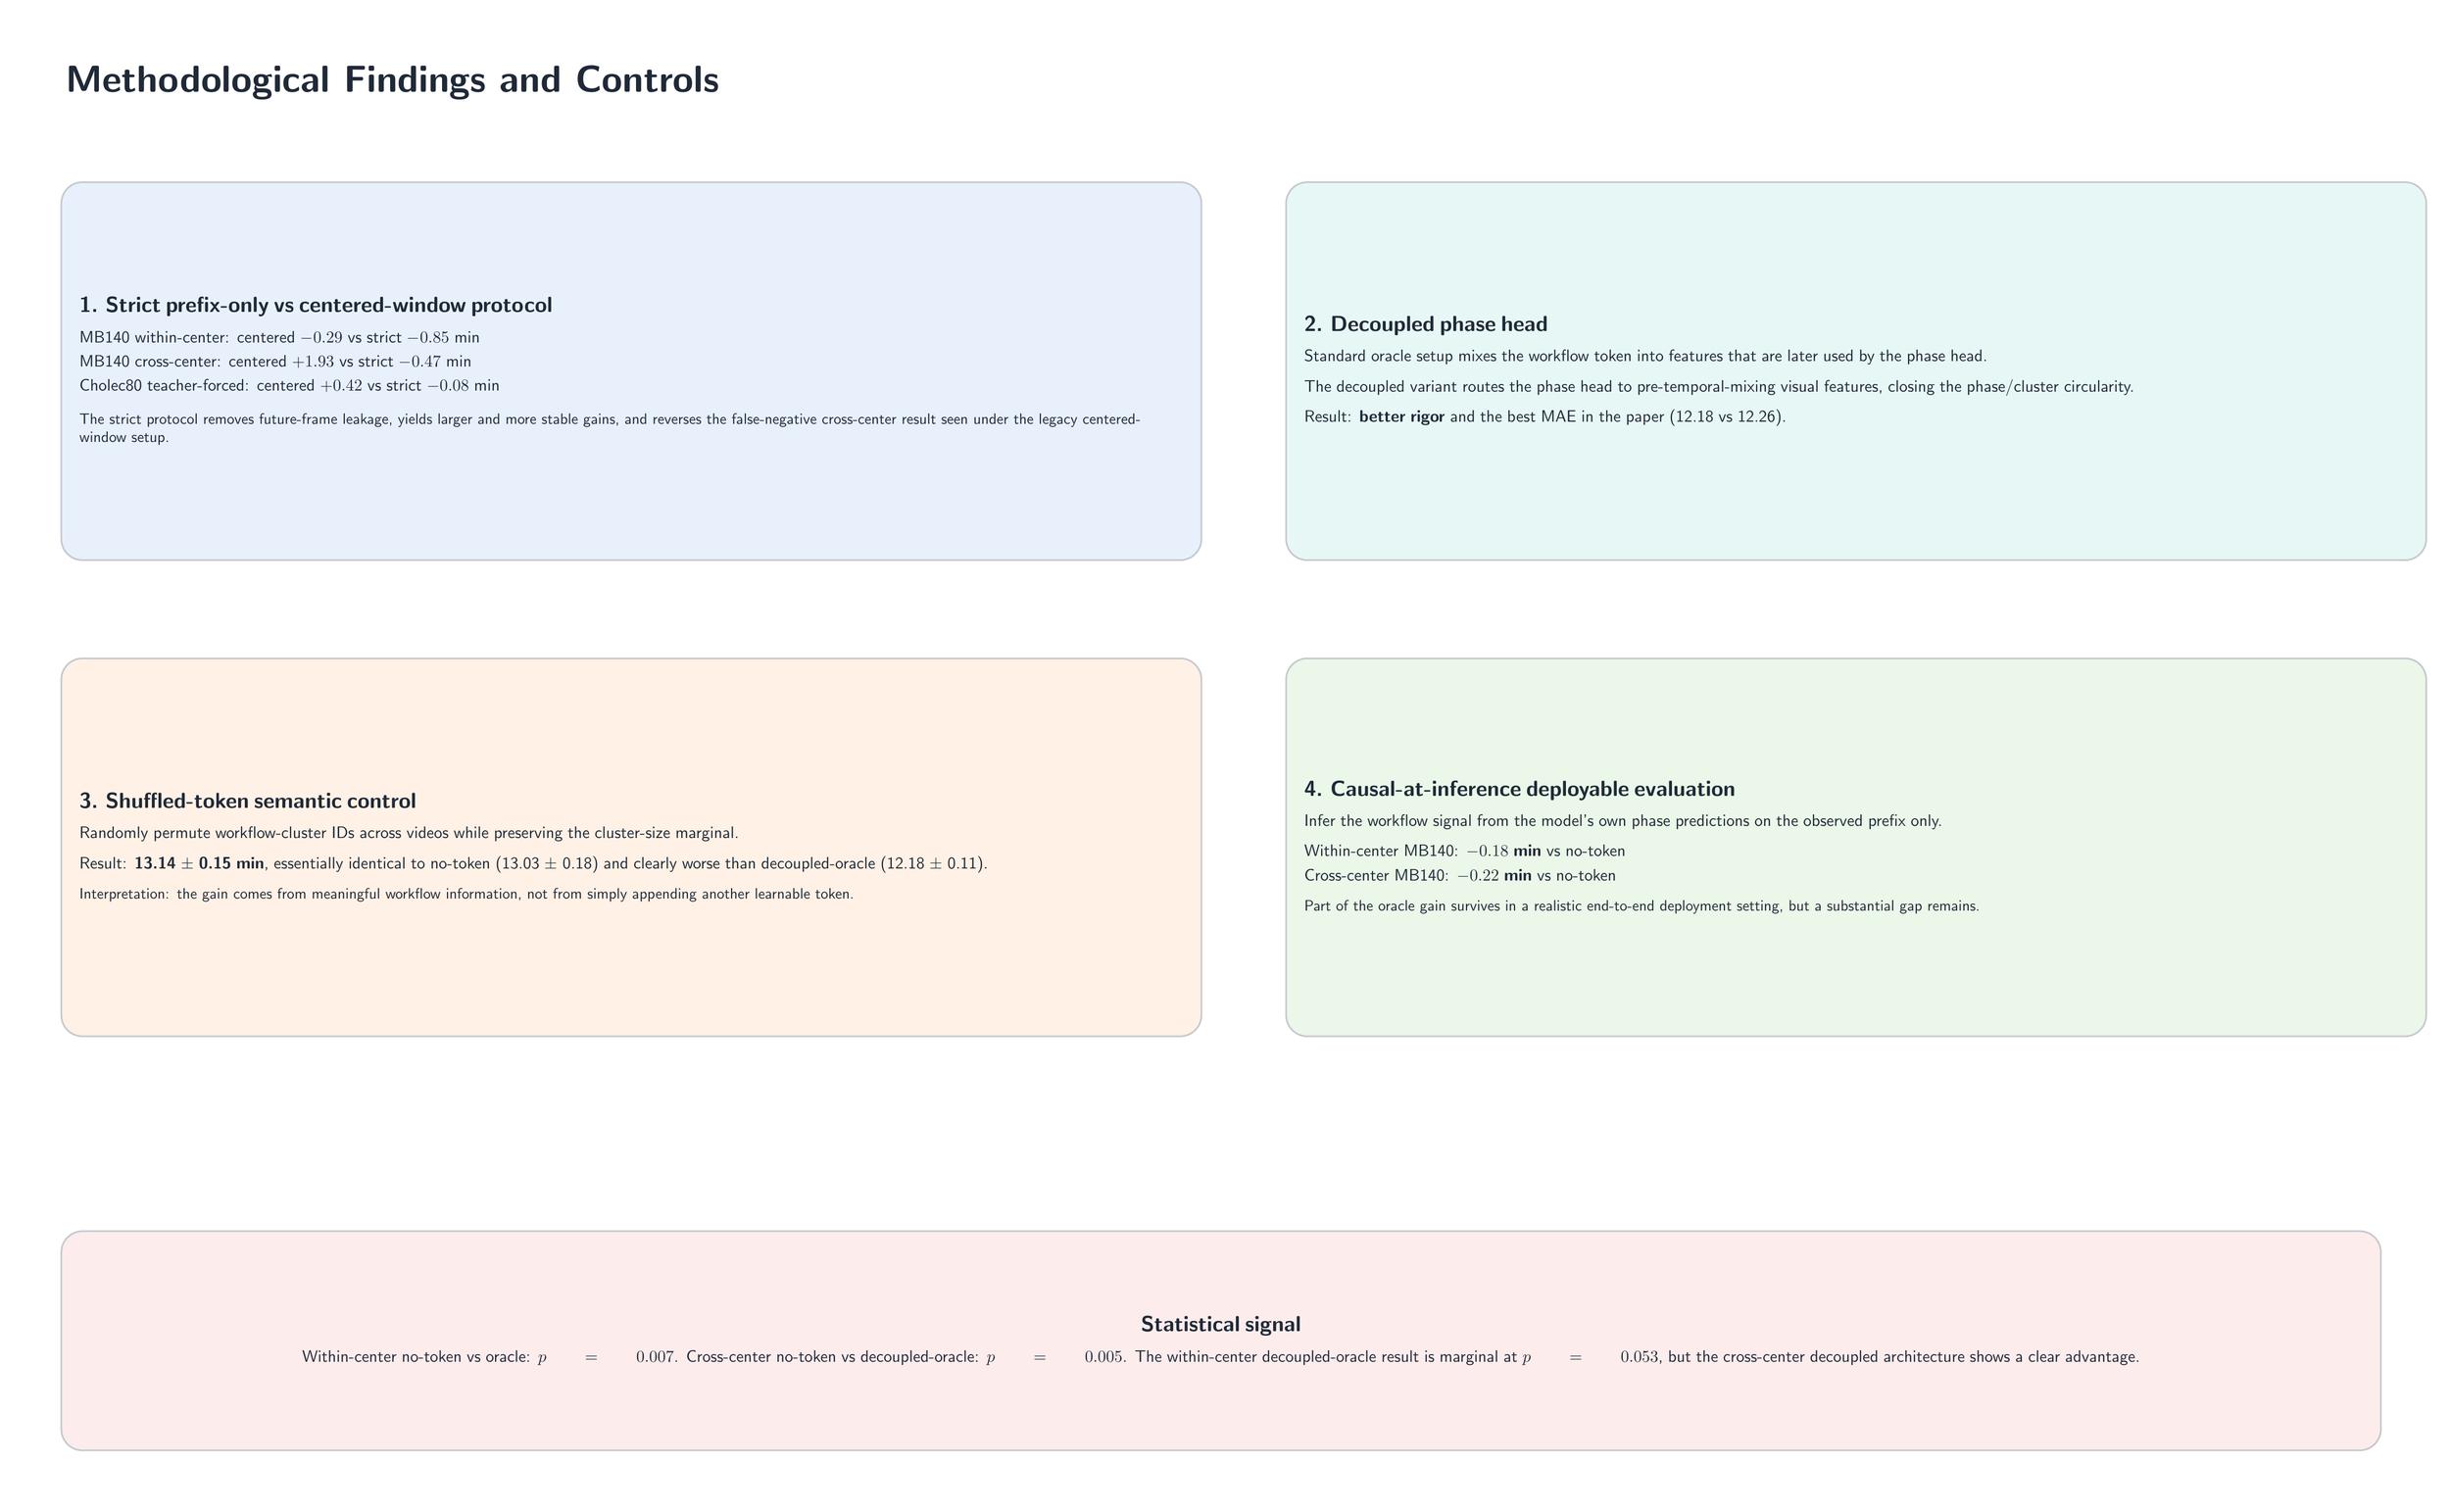
\begin{tikzpicture}[x=1pt,y=1pt]
\useasboundingbox (0,0) rectangle (1600,980);

\node[title, anchor=north west] at (30,950)
{Methodological Findings and Controls};

\node[bluebox, text width=730pt, minimum height=250pt, anchor=north west] at (30,870) {
{\subtitle 1. Strict prefix-only vs centered-window protocol}\par\vspace{8pt}
{\body MB140 within-center: centered \(-0.29\) vs strict \textbf{\(-0.85\)} min}\par\vspace{4pt}
{\body MB140 cross-center: centered \textbf{\(+1.93\)} vs strict \textbf{\(-0.47\)} min}\par\vspace{4pt}
{\body Cholec80 teacher-forced: centered \textbf{\(+0.42\)} vs strict \(-0.08\) min}\par\vspace{10pt}
{\smallbody The strict protocol removes future-frame leakage, yields larger and more stable gains, and reverses the false-negative cross-center result seen under the legacy centered-window setup.}
};

\node[tealbox, text width=730pt, minimum height=250pt, anchor=north west] at (840,870) {
{\subtitle 2. Decoupled phase head}\par\vspace{8pt}
{\body Standard oracle setup mixes the workflow token into features that are later used by the phase head.}\par\vspace{8pt}
{\body The decoupled variant routes the phase head to pre-temporal-mixing visual features, closing the phase/cluster circularity.}\par\vspace{8pt}
{\body Result: \textbf{better rigor} and the best MAE in the paper (12.18 vs 12.26).}
};

\node[orangebox, text width=730pt, minimum height=250pt, anchor=north west] at (30,555) {
{\subtitle 3. Shuffled-token semantic control}\par\vspace{8pt}
{\body Randomly permute workflow-cluster IDs across videos while preserving the cluster-size marginal.}\par\vspace{8pt}
{\body Result: \textbf{13.14 \(\pm\) 0.15 min}, essentially identical to no-token (13.03 \(\pm\) 0.18) and clearly worse than decoupled-oracle (12.18 \(\pm\) 0.11).}\par\vspace{8pt}
{\smallbody Interpretation: the gain comes from meaningful workflow information, not from simply appending another learnable token.}
};

\node[greenbox, text width=730pt, minimum height=250pt, anchor=north west] at (840,555) {
{\subtitle 4. Causal-at-inference deployable evaluation}\par\vspace{8pt}
{\body Infer the workflow signal from the model's own phase predictions on the observed prefix only.}\par\vspace{8pt}
{\body Within-center MB140: \textbf{\(-0.18\) min} vs no-token}\par\vspace{4pt}
{\body Cross-center MB140: \textbf{\(-0.22\) min} vs no-token}\par\vspace{8pt}
{\smallbody Part of the oracle gain survives in a realistic end-to-end deployment setting, but a substantial gap remains.}
};

\node[redbox, text width=1510pt, minimum height=145pt, anchor=south west, align=center] at (30,30) {
{\subtitle Statistical signal}\par\vspace{8pt}
{\body Within-center no-token vs oracle: \(p=0.007\). Cross-center no-token vs decoupled-oracle: \(p=0.005\). The within-center decoupled-oracle result is marginal at \(p=0.053\), but the cross-center decoupled architecture shows a clear advantage.}
};

\end{tikzpicture}
\end{document}
